% =====================================================================
%  O Espírito Santo como economia-plataforma
%  Felipe Carvalho — PPGEco/UFES
%  Análise de Insumo-Produto — Prof. Dr. Celso Bissoli Sessa — 2026/1
%
%  Números reproduzíveis a partir de pesquisa/ (MIP-ES-BR e interestadual
%  2008; WIOD 2014). Convenção de spillover/feedback: Miller-Blair (V3).
% =====================================================================
\documentclass[11pt,a4paper]{article}
\usepackage[utf8]{inputenc}
\usepackage[T1]{fontenc}
\renewcommand{\abstractname}{Resumo}
\renewcommand{\refname}{Referências}
\usepackage{amsmath,amssymb}
\usepackage{booktabs}
\usepackage{graphicx}
\usepackage{geometry}
\usepackage{xcolor}
\usepackage{framed}
\usepackage[round,authoryear]{natbib}
% Citações no padrão ABNT NBR 10520 (autor-data): (SOBRENOME, ano) e SOBRENOME (ano).
\bibpunct{(}{)}{;}{a}{,}{,}
\usepackage[hidelinks]{hyperref}
\geometry{margin=2.5cm}
\graphicspath{{../pesquisa/outputs/}{../figuras/}}
\definecolor{boxbg}{RGB}{246,243,234}\colorlet{shadecolor}{boxbg}

\title{\textbf{O Espírito Santo como economia-plataforma}\\[2pt]
\large Encadeamentos, vazamento de multiplicadores e a assimetria
\emph{spillover}--\emph{feedback} na cadeia inter-regional de valor
(MIP ES\,$\times$\,Brasil, 2008; WIOD, 2014)}
% ---------------------------------------------------------------------
% ATENÇÃO: preencher ORCID e e-mail acadêmico antes de enviar ao professor.
% ---------------------------------------------------------------------
\author{Felipe Carvalho\\
\small ORCID: 0000-0000-0000-0000\\
\small Programa de Pós-Graduação em Economia (PPGEco)\\
\small Universidade Federal do Espírito Santo (UFES), Vitória, ES, Brasil\\
\small \texttt{felipe.carvalho@edu.ufes.br}}
\date{julho de 2026}

\begin{document}
\maketitle
\thispagestyle{empty}

\begin{abstract}
\noindent
Este artigo propõe a leitura da economia do Espírito Santo (ES) como uma
\emph{economia-plataforma}: pequena, hiperaberta e estruturada em torno de
setores cuja demanda final se realiza fora do estado. A partir de uma matriz
insumo-produto inter-regional ES\,$\times$\,restante do Brasil para 2008
(26 setores por região; safra anterior ao rompimento de Fundão em 2015) e de
uma matriz interestadual das 27 unidades da
federação, aplica-se o modelo de Isard para (i) decompor o multiplicador de
produção de cada setor capixaba em parcela \emph{retida} e parcela
\emph{vazada}; (ii) isolar a assimetria entre o efeito \emph{spillover} e o
efeito \emph{feedback}; e (iii) rastrear o \emph{destino} geográfico do
vazamento. Em média, \textbf{24,9\%} do multiplicador de produção capixaba
vaza para fora do estado. Uma injeção de R\$\,51,5 bilhões na demanda final
do ES transborda R\$\,18,2 bilhões de produção para o restante do país, mas
o \emph{feedback} de volta é de apenas R\$\,164 milhões (\textbf{0,32\%}): a
interdependência é praticamente unilateral. O destino do vazamento é
concentrado --- o \textbf{Sudeste (excluído o ES) absorve 65\%} do
\emph{spillover}, e o núcleo São Paulo--Rio de Janeiro, 52,5\%. Uma camada de
cadeias globais de valor (WIOD 2014) situa a pauta exportadora capixaba com
\emph{upstreamness} de \textbf{3,12} (contra 1,91 do Brasil), com a mineração
no percentil 99 global. O mapa do vazamento é, simultaneamente, um mapa de
fragilidade estrutural e de oportunidade de adensamento de cadeia.

\vspace{0.6em}
\noindent\textbf{Palavras-chave:} insumo-produto; modelos inter-regionais;
vazamento de multiplicador; \emph{spillover} e \emph{feedback};
economia-plataforma; Espírito Santo.

\noindent\textbf{Códigos JEL:} R15; D57; C67.
\end{abstract}

\renewcommand{\abstractname}{Abstract}
\begin{abstract}
\noindent
This paper reads the economy of Espírito Santo (ES), Brazil, as a
\emph{platform economy}: small, hyper-open and organised around sectors whose
final demand is realised outside the state. Drawing on an interregional
input-output matrix for ES\,$\times$\,rest of Brazil for 2008 (26 sectors per
region; a vintage prior to the 2015 Fundão tailings-dam collapse) and on an
interstate matrix covering the 27 federal units, we apply the Isard model to
(i) decompose each sector's output multiplier into a \emph{retained} and a
\emph{leaked} share; (ii) isolate the asymmetry between \emph{spillover} and
\emph{feedback} effects; and (iii) trace the geographical \emph{destination} of
the leakage. On average, \textbf{24.9\%} of the state's output multiplier leaks
out. An injection of R\$\,51.5 billion into ES final demand spills R\$\,18.2
billion of output over to the rest of the country, whereas the feedback back to
ES is merely R\$\,164 million (\textbf{0.32\%}): interdependence is virtually
one-directional. The destination is highly concentrated --- the
\textbf{Southeast, excluding ES, absorbs 65\%} of the spillover, and the
São Paulo--Rio de Janeiro core alone 52.5\%. A global value chain layer
(WIOD 2014) places the state's export basket at an \emph{upstreamness} of
\textbf{3.12} (against 1.91 for Brazil), with mining in the 99th global
percentile. The map of leakage is simultaneously a map of structural fragility
and of opportunities for deepening local value chains.

\vspace{0.6em}
\noindent\textbf{Keywords:} input-output analysis; interregional models;
multiplier leakage; spillover and feedback; platform economy; Espírito Santo.

\noindent\textbf{JEL codes:} R15; D57; C67.
\end{abstract}
\renewcommand{\abstractname}{Resumo}

% =====================================================================
\section{Introdução}
\label{sec:intro}
Em 2008 o Espírito Santo respondia por cerca de 2\% do produto nacional, mas
sua estrutura produtiva é atípica: pequena, hiperaberta e concentrada em
setores cuja demanda final se realiza \emph{fora} do estado --- minério de
ferro e pelotização, siderurgia, celulose, petróleo e rochas ornamentais.
Este artigo testa a hipótese de que o ES pode ser descrito, com utilidade
analítica, como uma \emph{economia-plataforma} e responde a três perguntas:
(i) quanto do multiplicador capixaba fica e quanto vaza; (ii) \emph{para
onde} vaza; e (iii) o que o destino desse multiplicador revela sobre a
posição do estado nas cadeias de valor. A contribuição é levar a leitura do
vazamento da dimensão bi-regional (ES \emph{versus} resto do Brasil) à
dimensão \emph{interestadual}, identificando os estados que absorvem o
encadeamento que escapa do ES. A fotografia estrutural é de 2008, anterior ao
rompimento de Fundão (2015), o que circunscreve seu alcance temporal
(§\ref{sec:limites}).

Essa agenda conversa diretamente com três tradições, revisadas na
Seção~\ref{sec:revisao}: a literatura brasileira de insumo-produto regional,
que oferece o arcabouço de regionalização; a formulação de Isard e
Miller-Blair, que permite decompor o efeito externo em \emph{spillover} e
\emph{feedback}; e a literatura de cadeias globais de valor, que situa a pauta
na dimensão montante/jusante. O artigo combina essas três camadas para mostrar
que o ES vaza muito, vaza para poucos destinos e retorna pouco.

O texto está organizado como segue. A Seção~\ref{sec:revisao} revisa o estado
da arte da aplicação do modelo insumo-produto ao problema do vazamento
regional. A Seção~\ref{sec:metodo} descreve a matriz utilizada e apresenta
formalmente as equações do modelo. A Seção~\ref{sec:resultados} reporta os
resultados; a Seção~\ref{sec:discussao} os confronta com a literatura; as
Seções~\ref{sec:limites} a~\ref{sec:conclusao} declaram limites, agenda e
conclusões.

% =====================================================================
\section{Revisão de Literatura}
\label{sec:revisao}

\subsection{Insumo-produto regional no Brasil: do nacional ao inter-regional}
A análise insumo-produto regional brasileira enfrenta uma restrição
estrutural: o país publica matrizes \emph{nacionais} com regularidade, mas não
um sistema inter-regional observado. A resposta consolidada da literatura foi
desenvolver métodos de estimação que preservem consistência com o agregado
nacional. \citet{guilhoto2005estimacao} são a referência dessa tradição ao
mostrarem como estimar matrizes a partir de dados preliminares das contas
nacionais, viabilizando o uso de safras mais recentes sem esperar a matriz
definitiva do IBGE. Sobre essa base, \citet{haddad2017iioas} constroem o
sistema inter-regional das 27 unidades da federação pelo método IIOAS,
combinando as tabelas de recursos e usos com técnicas não-censitárias.

Antes desse esforço nacional, a literatura brasileira já acumulara
\emph{matrizes bi-regionais} estado\,$\times$\,resto do país.
\citet{domingues2002matriz} estimam a matriz Minas Gerais/Resto do Brasil e a
estendem para exportações; \citet{porsse2008matriz} fazem o mesmo para o Rio
Grande do Sul, documentando transbordamentos do estado para o restante do país
mais intensos que o retorno --- com vazamento menor nos setores
agroindustriais e maior nos ramos metal-mecânicos. Essas matrizes bi-regionais
estabeleceram o achado que este artigo retoma: a interdependência
inter-regional brasileira é assimétrica, e o sentido dessa assimetria depende
da composição setorial do estado. O que elas não fazem --- e o que a matriz
interestadual permite --- é desagregar \emph{para onde} o encadeamento escoa.

\subsection{Métodos não-censitários de regionalização}
Como raramente se observam fluxos de comércio inter-regionais, a matriz
regional é quase sempre \emph{estimada}. \citet{round1983nonsurvey} organizou
criticamente esse campo, distinguindo as famílias de técnicas e alertando para
o fato de que a escolha do método não é neutra sobre os resultados. Três
famílias são relevantes aqui.

A primeira é a dos \emph{quocientes locacionais}, que inferem a
auto-suficiência regional a partir da participação setorial relativa. Sua
variante mais usada, a FLQ e o refinamento AFLQ, corrige o viés de tamanho
regional: \citet{flegg2016evaluating} avaliam essas fórmulas contra dados
observados e mostram que os coeficientes estimados são sensíveis ao parâmetro
de ajuste --- uma sensibilidade que este artigo declara na
Seção~\ref{sec:limites}. A segunda é o método CHARM, que corrige o
\emph{cross-hauling} (comércio simultâneo de ida e volta do mesmo produto)
sistematicamente ignorado pelos quocientes \citep{tobben2015charm}. A terceira
é a das abordagens \emph{gravitacionais}, que modelam o fluxo entre regiões em
função de massa econômica e distância; \citet{riddington2006comparison}
comparam modelo gravitacional, levantamento censitário e quocientes
locacionais, concluindo que as formulações gravitacionais tendem a reproduzir
melhor os fluxos observados.

O IIOAS filia-se a essa terceira família \citep{haddad2017iioas}: na ausência
de fluxos observados, combina os coeficientes da matriz nacional --- sob a
hipótese de tecnologia e preferências comuns, na tradição de Chenery-Moses ---
a um modelo gravitacional calibrado por tempos de viagem entre as UFs. A opção
por ele neste artigo é deliberada e não metodológica em sentido estrito: é o
método com que a matriz interestadual aqui mobilizada foi efetivamente
construída, de modo que usá-lo garante consistência com o substrato empírico.

\subsection{Vazamento, \emph{spillover} e \emph{feedback}}
O aparato para separar o que fica do que escapa remonta a
\citet{isard1951}, que formulou o modelo inter-regional em que a economia do
espaço é representada por blocos intra e inter-regionais, e à sistematização
de \citet{millerblair2009}, hoje a referência canônica da partição da inversa
de Leontief. A distinção conceitual decisiva é entre o \emph{spillover} --- a
produção que a demanda de uma região induz nas demais --- e o \emph{feedback},
a parcela que retorna à região de origem após circular fora dela.

A magnitude esperada desse retorno é, ela própria, objeto de literatura.
\citet{miller1966} mostrou, em resultados preliminares que se tornaram
referência, que os efeitos de retorno inter-regional tendem a ser pequenos
para regiões pequenas e abertas. Esse é um ponto importante para a
interpretação: um \emph{feedback} próximo de zero não é, por si só, um achado
surpreendente para um estado do porte do ES --- é aproximadamente o que a
mecânica do modelo prediz. O que exige explicação, e o que este artigo
persegue, é a \emph{geografia} do transbordamento.

Aplicações brasileiras dão a medida do padrão. \citet{peixoto2013metodologia},
ao decompor o agronegócio gaúcho em elos a montante, produção rural e elos a
jusante, estimam que apenas 0,4\% do valor adicionado do agronegócio do
restante do Brasil decorre de elos inter-regionais com o Rio Grande do Sul,
ante 7,9\% do valor gaúcho que decorre de elos com o restante do país --- uma
assimetria de captura da mesma natureza da que se documenta aqui. Já
\citet{figueiredo2004agriculture}, para Mato Grosso, mostram que a soja, setor
exportador dominante, gera apenas 8 empregos diretos por R\$ 1 milhão de
demanda final, ante 31 indiretos e 72 com o efeito induzido, e que seus
setores-chave são quase todos primário-exportadores: baixa retenção direta com
alta propagação, o mesmo desenho que o ES exibe pelo lado do minério.

\subsection{Posição em cadeias de valor}
A terceira camada vem da literatura de cadeias globais de valor.
\citet{antras2012measuring} propõem o índice de \emph{upstreamness}, que mede
a distância média de um setor em relação ao uso final e permite classificar
economias como fornecedoras a montante ou montadoras a jusante. Sua aplicação
requer uma base multirregional: a \emph{World Input-Output Database}
\citep{timmer2015wiod} tornou-se o instrumento padrão, ainda que
\citet{tukker2013global} alertem para as escolhas de construção que separam as
diferentes bases MRIO e para o tratamento devido a entradas negativas, e que
\citet{oecd2019tiva} documentem como a demanda final implícita incorpora
variação de estoques e discrepância estatística. No Brasil,
\citet{araujojunior2018cgv} aplica esse instrumental à inserção do país em
cadeias globais. O ponto que a literatura de CGV \emph{não} resolve, e que
motiva a combinação proposta neste artigo, é onde se concentra o valor
capturado \emph{internamente} ao país --- questão que só o recorte
interestadual responde.

% =====================================================================
\section{Metodologia}
\label{sec:metodo}

\subsection{Descrição da matriz: ano, fonte, setorização e agregação}
\label{sec:dados}
A espinha empírica combina três fontes, todas processadas por rotinas
reprodutíveis (\texttt{pesquisa/}): (a) a matriz insumo-produto
\textbf{inter-regional ES\,$\times$\,restante do Brasil} para 2008, com 26
setores por região (52 ao todo), R\$ milhões correntes, contábil e balanceada,
acompanhada do vetor de pessoal ocupado; (b) a matriz \textbf{interestadual}
das 27 UFs (26 setores por UF) para 2008, que permite a decomposição do destino
do vazamento; e (c) a \emph{World Input-Output Database} (WIOD) de 2014 --- 44
regiões e 56 setores --- para a camada de cadeias globais de valor
\citep{timmer2015wiod}. A construção das matrizes regionais segue a tradição
brasileira de regionalização da matriz nacional \citep{guilhoto2005estimacao} e
de estimação de fluxos inter-regionais pelo método IIOAS
\citep{haddad2017iioas}, discutidos na Seção~\ref{sec:revisao}.

A \textbf{agregação} adotada é a de 26 setores por região, herdada da matriz
inter-regional de origem; ela preserva separadamente os ramos que importam
para a tese (mineração, metalurgia, madeira/papel, refino) e agrega os
serviços em blocos amplos. Para a camada de CGV, a concordância entre os 26
setores da matriz brasileira e os 56 do WIOD é aproximada e feita setor a
setor, limitação declarada na Seção~\ref{sec:limites}. Todos os resultados
reportados são reprodutíveis a partir dos artefatos versionados e conferidos
na planilha de auditoria descrita no Apêndice~\ref{ap:auditoria}.

\subsection{Modelo formal}
Sejam $L$ (ES) e $M$ (restante do Brasil) duas regiões. A matriz de
coeficientes técnicos e a inversa de Leontief $L=(I-A)^{-1}$ particionam-se em
blocos intra e inter-regionais \citep{millerblair2009,isard1951}:
\begin{equation}
A=\begin{bmatrix} A^{LL} & A^{LM}\\ A^{ML} & A^{MM}\end{bmatrix},
\qquad
\begin{bmatrix} x^{L}\\ x^{M}\end{bmatrix}
=(I-A)^{-1}\begin{bmatrix} f^{L}\\ f^{M}\end{bmatrix}
=\begin{bmatrix} L^{LL} & L^{LM}\\ L^{ML} & L^{MM}\end{bmatrix}
\begin{bmatrix} f^{L}\\ f^{M}\end{bmatrix},
\label{eq:isard}
\end{equation}
com $A=Z\hat{x}^{-1}$. Resolvendo para a região $L$ obtém-se a forma reduzida
com o termo de \emph{feedback} explícito:
\begin{equation}
x^{L}
=\underbrace{(I-A^{LL})^{-1}}_{\text{intra}}f^{L}
\;+\;\underbrace{\big[(I-A^{LL}-A^{LM}(I-A^{MM})^{-1}A^{ML})^{-1}-(I-A^{LL})^{-1}\big]f^{L}}_{\text{feedback}}.
\label{eq:feedback}
\end{equation}

\paragraph{Decomposição do multiplicador de produção.}
$O_j=\sum_i \ell_{ij}$ separa-se em parcela retida e vazada,
$O^{L}_j=\sum_{i\in L}\ell_{ij}$ e $O^{M}_j=\sum_{i\in M}\ell_{ij}$, com
vazamento relativo $O^{M}_j/O_j$.

\paragraph{Multiplicador de emprego.}
$E_j=\sum_i w_i\,\ell_{ij}$, com coeficiente de trabalho
$w_i=\text{ocupações}_i/x_i$; o vazamento de emprego é a parcela de $E_j$
realizada em $M$.

\paragraph{\emph{Spillover} e \emph{feedback}.}
Injeta-se a demanda final do ES por produtos do ES, $f^{L}$ (com $f^{M}=0$);
mede-se a produção induzida em $M$ via
$x^{M}=(I-A^{MM})^{-1}A^{ML}x^{L}$ (\emph{spillover}) e o retorno a $L$ pelo
segundo termo de~\eqref{eq:feedback} (\emph{feedback}). Na matriz interestadual,
$x^{M}$ é desagregado por unidade da federação.

\paragraph{\emph{Upstreamness}.}
A posição em cadeias de valor usa o índice de \citet{antras2012measuring},
$U=(I-G)^{-1}\mathbf{1}$, com $G_{ij}=z_{ij}/x_i$; a \emph{upstreamness} da
pauta do ES pondera a $U$ setorial do Brasil (WIOD 2014, \citealp{timmer2015wiod})
pela composição das
exportações capixabas.

% =====================================================================
\section{Resultados}
\label{sec:resultados}

\subsection{Vazamento do multiplicador de produção}
Em média, 24,9\% do multiplicador de produção capixaba vaza para fora do
estado\footnote{Trata-se da \emph{média simples} entre os 26 setores,
comparável à média setorial de \citet{haddad2017iioas}. A média
\emph{ponderada pela produção} do ES é 22,8\% --- valor reportado na
Tabela~\ref{tab:cluster} e na Figura~\ref{fig:cluster}, em que a ponderação
garante comparabilidade entre estados de tamanhos distintos. As duas medidas
descrevem o mesmo fenômeno sob agregações diferentes.} --- número convergente,
em safra e agregação distintas, com os 27,4\% estimados por
\citet{haddad2017iioas}. A distribuição setorial completa está na
Tabela~\ref{tab:setores}: serviços imobiliários quase não vazam (5,3\%),
enquanto alimentos vazam 37,4\%. No emprego, nos setores pesados metade ou
mais do trabalho puxado pela demanda capixaba realiza-se fora do ES --- refino
61,6\%, alimentos 56,5\%, madeira/papel 50,3\% e metalurgia 49,3\%.

\begin{table}[htbp]
\centering\small
\begin{tabular}{lrrrrr}
\toprule
Setor & $O_j$ & Vaz.\ prod.\ (\%) & Vaz.\ empr.\ (\%) & Lig.\ trás & Lig.\ frente\\
\midrule
Imobiliário/aluguel & 1,15 & 5,2 & 12,3 & 0,64 & 0,65\\
Educação & 1,31 & 11,6 & 7,1 & 0,73 & 0,57\\
Financeiro/seguros & 1,47 & 12,8 & 20,6 & 0,82 & 1,21\\
Adm. pública & 1,43 & 15,0 & 16,0 & 0,80 & 0,60\\
Comércio & 1,42 & 16,0 & 7,6 & 0,79 & 0,91\\
Serviços privados & 1,50 & 17,9 & 8,4 & 0,84 & 1,18\\
Saúde & 1,54 & 19,1 & 14,9 & 0,86 & 0,57\\
Eletricidade/gás/água & 1,83 & 21,0 & 28,4 & 1,02 & 1,32\\
Agricultura/silvicultura & 1,45 & 21,6 & 9,9 & 0,81 & 0,93\\
Mineração & 1,64 & 22,7 & 42,4 & 0,91 & 1,23\\
Máquinas/equip. & 2,00 & 24,9 & 26,5 & 1,12 & 0,93\\
Construção & 1,70 & 25,5 & 16,1 & 0,95 & 0,69\\
Material de transporte & 2,10 & 26,1 & 29,7 & 1,17 & 1,11\\
Refino/coque/álcool & 2,11 & 27,8 & 61,6 & 1,18 & 1,17\\
Têxtil/vestuário & 1,87 & 28,1 & 17,8 & 1,04 & 0,82\\
Metalurgia & 1,96 & 29,2 & 49,2 & 1,09 & 1,30\\
Químicos/farmacêuticos & 2,10 & 29,4 & 41,2 & 1,17 & 1,71\\
Mat. elétrico/eletrônicos & 1,99 & 29,8 & 34,1 & 1,11 & 1,12\\
Pecuária e pesca & 1,64 & 30,2 & 19,4 & 0,91 & 1,08\\
Transporte/armazenagem & 1,77 & 30,3 & 23,1 & 0,99 & 1,22\\
Indústrias diversas & 1,84 & 30,5 & 16,3 & 1,02 & 0,74\\
Min. não-metálicos & 1,90 & 30,6 & 28,2 & 1,06 & 1,09\\
Alojamento/alimentação & 1,76 & 31,9 & 22,2 & 0,98 & 0,75\\
Madeira/papel & 1,96 & 35,8 & 50,3 & 1,09 & 0,84\\
Borracha/plástico & 2,05 & 36,8 & 32,9 & 1,14 & 1,26\\
Alimentos/bebidas/fumo & 2,31 & 37,4 & 56,5 & 1,29 & 0,78\\
\midrule
\textbf{Média (simples)} & 1,76 & 24,9 & 26,6 & 0,98 & 0,99\\
\textbf{Média (ponderada)} & 1,66 & 22,9 & 26,0 & 0,92 & 1,01\\
\bottomrule
\end{tabular}

\caption{Multiplicador de produção ($O_j$), vazamentos de produção e de emprego e
ligações de Rasmussen-Hirschman dos 26 setores do ES, ordenados pelo vazamento do
multiplicador de produção. Vazamento médio: simples 24,9\% (comparável a
\citealp{haddad2017iioas}); ponderado pela produção 22,9\% (bi-regional; 22,8\% na
matriz interestadual, Tabela~\ref{tab:cluster}). Fonte: \texttt{12\_tab\_setores.py}
sobre \texttt{outputs/es\_setores\_resultados.csv}.}
\label{tab:setores}
\end{table}

% (vazamento de emprego incorporado à Tabela~\ref{tab:setores})

\subsection{A assimetria \emph{spillover}/\emph{feedback}}
Uma injeção de R\$\,51,5 bilhões na demanda final do ES (por produtos do ES)
transborda R\$\,18,2 bilhões de produção para o restante do país, mas o
\emph{feedback} de volta é de apenas R\$\,164 milhões --- 0,32\% da injeção
(Figura~\ref{fig:sankey}). A interdependência é praticamente unilateral: do
total de produção que a demanda capixaba coloca em movimento, 78\% fica no
ES e o restante escoa para fora, quase sem retorno.

\begin{figure}[ht]
\centering

\includegraphics[width=.92\linewidth]{es_sankey.png}
\caption{Destino do \emph{spillover} do ES (R\$\,18,1 bilhões --- os 22\% da produção
que vazam), estratificado por macrorregião e estado. O núcleo SP/RJ (azul) absorve a
maior parte; Minas Gerais e os pares do cluster aparecem em verde e o restante em cinza.
A produção retida no ES (78\%) e o \emph{feedback} de volta ($\approx$0,3\%) constam do
subtítulo da figura.}
\label{fig:sankey}
\end{figure}

\subsection{Para onde vaza: a geografia interestadual}
A matriz interestadual revela que o vazamento não se dispersa
aleatoriamente: o \textbf{Sudeste (excluído o ES) absorve 65,4\%} do
\emph{spillover} capixaba --- São Paulo 37,8\%, Rio de Janeiro 14,7\% e Minas
Gerais 12,9\% (Figura~\ref{fig:destino}). O ES alimenta sobretudo seus
vizinhos mais ricos; o encadeamento que escapa é capturado a jusante por
economias mais diversificadas.

\begin{figure}[ht]
\centering
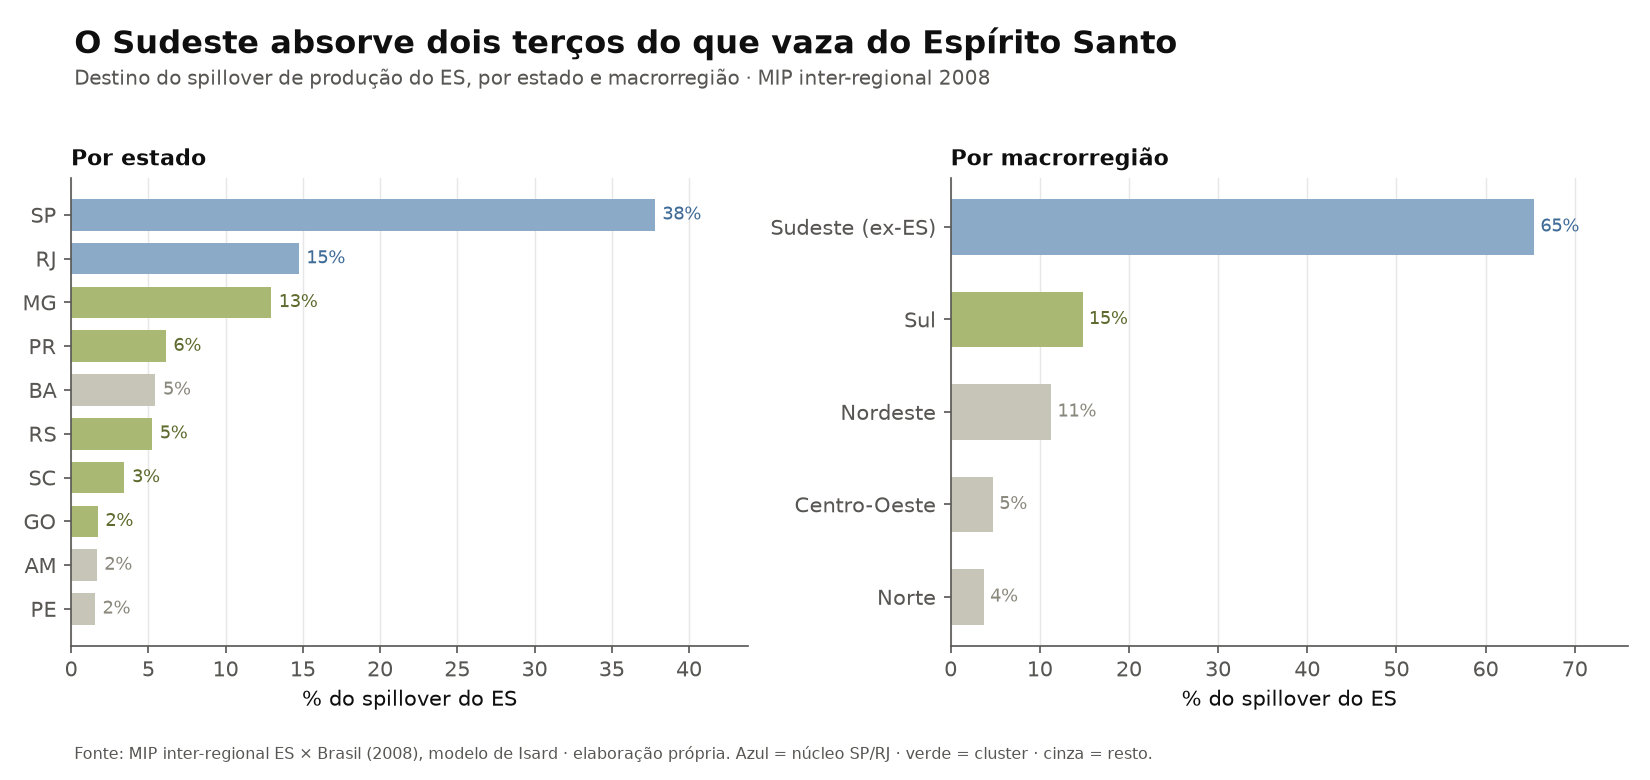
\includegraphics[width=.95\linewidth]{es_spillover_destino.png}
\caption{Destino do \emph{spillover} do ES por estado e por macrorregião.}
\label{fig:destino}
\end{figure}

\subsection{O ES num cluster de estados dinâmicos}
O ES integra um conjunto de oito estados de crescimento acima da média e
sub-cobertos pelo mercado de capitais (SC, PR, ES, MG, RS, GO, MT, MS), que
exclui justamente o núcleo SP/RJ.\footnote{Agrupamento na esteira da leitura
de mercado da Apex Partners; aqui tratado como \emph{cluster de comparação},
sem caráter de regionalização oficial.} Esse cluster respondia por 33,9\% do
PIB em 2008. Dentro dele, o ES é o estado mais aberto depois das fronteiras
agro-minerais e o segundo mais intensivo em setores de base (36,4\% da
produção; Tabela~\ref{tab:cluster}); 52,5\% de seu \emph{spillover} vai ao
núcleo SP+RJ contra 31,5\% aos demais pares (Figura~\ref{fig:cluster}). A
leitura insumo-produto é a contraparte estrutural da tese de sub-cobertura de
capital: o elo produtivo flui ao centro, o capital não retorna. Embora a
delimitação do grupo seja externa (crescimento acima da média e sub-cobertura de
capital), o cluster tem assinatura estrutural replicável no próprio dado: seis dos
oito estados situam-se acima da mediana nacional tanto em abertura (21,8\%) quanto em
base/\emph{commodity} (21,0\%) --- e todos os oito acima da mediana de base ---,
enquanto o núcleo SP/RJ situa-se abaixo; o agrupamento não é, pois, arbitrário do
ponto de vista da estrutura produtiva, ainda que não derive de regionalização oficial.
O desenho \emph{commodity}-exportador desse cluster já fora documentado em
estudos inter-regionais de pares --- notadamente em Mato Grosso, o estado de
maior vazamento da Tabela~\ref{tab:cluster}, cujo perfil de baixa retenção
direta e alta propagação \citep{figueiredo2004agriculture} é o mesmo que o ES
exibe pelo lado do minério (Seção~\ref{sec:revisao}).

\begin{table}[ht]
\centering
\begin{tabular}{lrrrl}
\toprule
Estado & PIB (\%) & Vazamento (\%) & Base/\emph{commodity} (\%) & Setor dominante\\
\midrule
\textbf{ES} & 2,2 & 22,8 & \textbf{36,4} & Mineração\\
MG & 9,5 & 20,9 & 29,6 & Metalurgia\\
SC & 4,1 & 22,5 & 21,7 & Alimentos\\
PR & 6,0 & 22,3 & 28,0 & Alimentos\\
RS & 6,7 & 21,8 & 24,6 & Alimentos\\
GO & 2,6 & 25,1 & 32,8 & Alimentos\\
MT & 1,8 & 27,4 & 43,4 & Agricultura\\
MS & 1,1 & 25,7 & 30,1 & Alimentos\\
\midrule
SP \emph{(núcleo)} & 32,0 & 14,2 & 18,0 & Serviços\\
RJ \emph{(núcleo)} & 11,2 & 15,6 & 27,4 & Mineração\\
\bottomrule
\end{tabular}
\caption{O ES e os pares do cluster \emph{versus} o núcleo SP/RJ
(\texttt{outputs/cluster\_setorial.csv}).}
\label{tab:cluster}
\end{table}

\begin{figure}[ht]
\centering
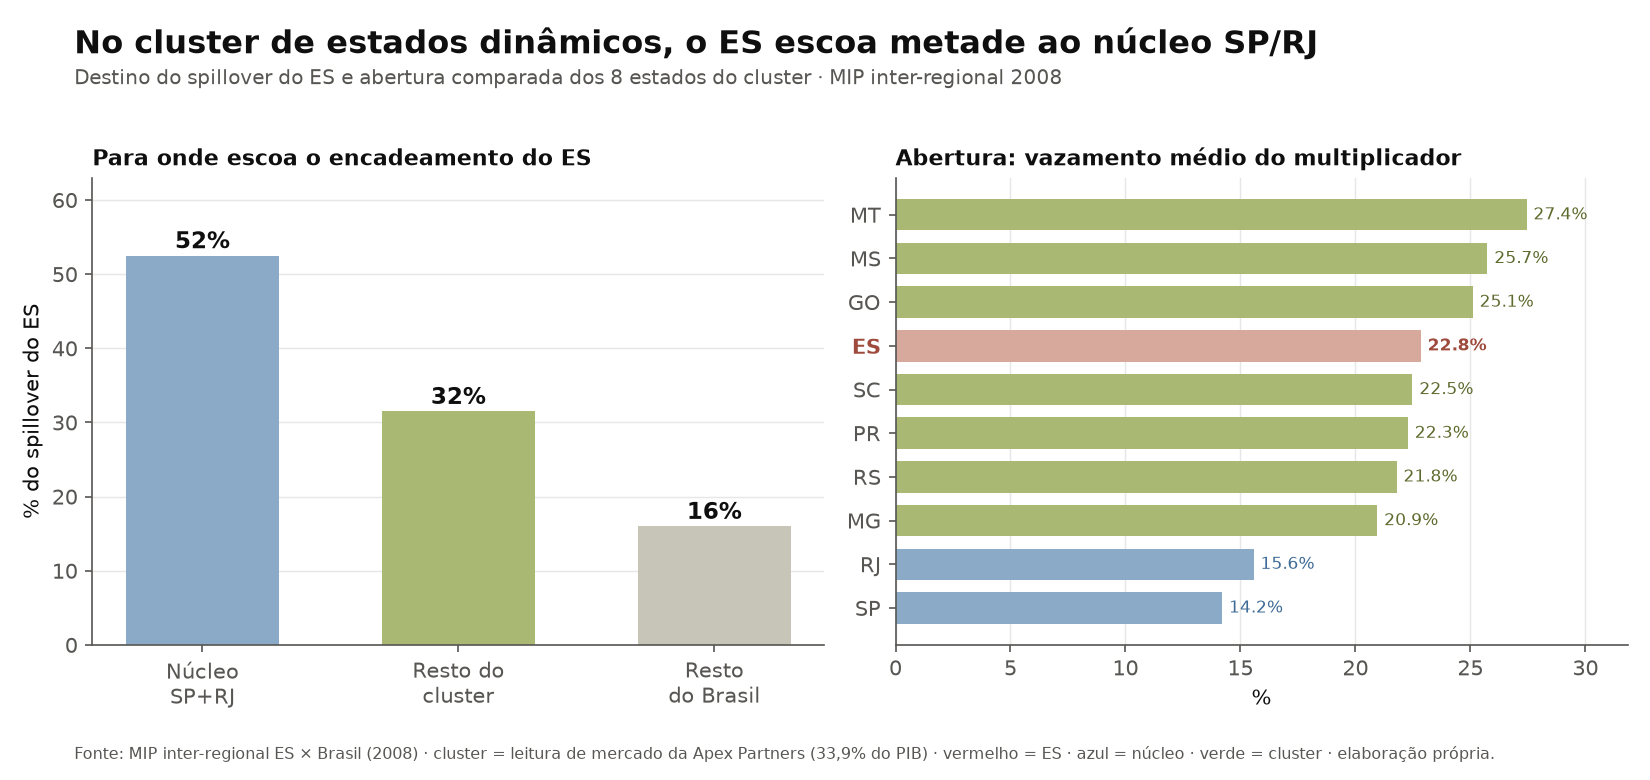
\includegraphics[width=.95\linewidth]{es_cluster.png}
\caption{Destino do \emph{spillover} do ES (núcleo \emph{vs} cluster \emph{vs}
resto) e abertura comparada dos estados do cluster e do núcleo.}
\label{fig:cluster}
\end{figure}

\subsection{Posição em cadeias globais de valor}
A pauta exportadora capixaba tem \emph{upstreamness} ponderada de
\textbf{3,12}, contra 1,91 do Brasil e 2,31 da média mundial, com a mineração
entre as mais a montante do mundo ($U=3,82$; 33\textordfeminine{} de 2.279
posições válidas do WIOD, percentil 99 após o tratamento de qualidade do
§\ref{sec:limites}; Figura~\ref{fig:upstream}). O ES supre insumos
primários e intermediários (mineração, metalurgia e celulose somam 71\% das
exportações); a captura de valor a jusante ocorre em outras regiões e países.
Esse posicionamento a montante tem contraparte na evidência nacional: a
assimetria de captura documentada por \citet{peixoto2013metodologia} para o
agronegócio gaúcho (Seção~\ref{sec:revisao}) é da mesma natureza da que o ES
revela na escala interestadual.

\begin{figure}[ht]
\centering

\includegraphics[width=.9\linewidth]{es_upstreamness.png}
\caption{\emph{Upstreamness} (Antràs-Chor) da pauta do ES, WIOD 2014: o estado
posiciona-se a montante da cadeia de valor.}
\label{fig:upstream}
\end{figure}

% =====================================================================
\section{Discussão}
\label{sec:discussao}
O resultado principal não deve ser lido como uma generalização universal sobre
estados exportadores, mas como uma evidência estrutural para o ES em 2008.
Nesse ponto, a contribuição é complementar à literatura: Haddad et al.
documentam a construção da matriz e a existência de vazamentos relevantes;
Guilhoto e Sesso Filho mostram como regionalizar a economia brasileira; Isard
e Miller-Blair fornecem o aparato para separar o retorno interno do efeito
externo; e Antràs-Chor situam a pauta na cadeia global. O passo adicional
deste trabalho é juntar essas quatro peças em uma mesma narrativa: a abertura
do ES não é apenas alta, ela é espacialmente concentrada e com baixo retorno.

O padrão é coerente com a evidência inter-regional brasileira revisada na
Seção~\ref{sec:revisao}: tanto a matriz Rio Grande do Sul--Restante do Brasil
de \citet{porsse2008matriz} quanto a matriz Minas Gerais--Resto do Brasil de
\citet{domingues2002matriz} já documentavam transbordamentos mais intensos que
o retorno. O resultado capixaba confirma a direção do achado e acrescenta
magnitude: a razão \emph{feedback}/injeção de 0,32\% é de uma ordem que torna
a interdependência, para fins práticos, unilateral. A contribuição própria,
porém, é de outra natureza --- é levar o achado do par bi-regional ao recorte
\emph{interestadual}, identificando \emph{para onde} escoa o encadeamento, algo
que as matrizes bi-regionais, por construção, não podem responder.

Convém separar o que é específico do ES do que é genérico a economias pequenas e
abertas. A pequenez do \emph{feedback} é, em parte, uma regularidade do método --- os
efeitos de retorno inter-regional tendem a ser pequenos para regiões pequenas e abertas
\citep{miller1966} ---, e a Tabela~2 de \citet{haddad2017iioas} mostra vários estados
com parcela inter-regional do multiplicador total na faixa do ES (MT 28,5\%, MS 29,7\%,
AM 25,2\%; ES 27,4\% --- métrica de Haddad, distinta do vazamento ponderado da
Tabela~\ref{tab:cluster}). O que o dado capixaba acrescenta não é, pois, a \emph{existência}
de vazamento --- esperada pelo porte ---, mas dois fatos que essa mecânica não prediz: a
\emph{concentração do destino} no Sudeste e no núcleo SP/RJ (65,4\% e 52,5\%) e a
\emph{posição a montante} da pauta específica. É na geografia do transbordamento e na
posição em cadeia, não na assimetria \emph{per se}, que reside a contribuição própria.

O mecanismo por trás da assimetria é direto. O ES é um \emph{hub} de passagem
de intermediários pesados; o choque de demanda vaza rapidamente para a
importação de insumos avançados e bens de consumo de SP e MG, mas as rodadas
seguintes de consumo do Sudeste quase não recorrem de volta às \emph{commodities}
brutas capixabas. Por isso o \emph{feedback} medido pela matriz é muito
pequeno em relação à injeção, ainda que não seja literalmente zero. O mapa do
vazamento é, ao mesmo tempo, um mapa de \emph{fragilidade} (setores que apenas
transitam pelo estado) e de \emph{oportunidade} (setores que retêm
multiplicador e adensam cadeia). A análise operacionaliza a noção de
``vocação local'', distinguindo quantitativamente os setores que aprofundam a
cadeia regional dos que apenas a atravessam.

% =====================================================================
\section{Limitações}
\label{sec:limites}
Três limites são declarados com franqueza. \textbf{(i) Gap temporal e quebra
estrutural:} a matriz base é de 2008; o ES sofreu choques desde então, o mais
drástico o rompimento da barragem de Fundão (2015), que paralisou a Samarco e
alterou o peso da extração e da pelotização. \textbf{(ii) Fluxos estimados:} os
fluxos inter-regionais e interestaduais são \emph{estimados} pelo método IIOAS
(não observados), de modo que os resultados de destino do vazamento carregam as
hipóteses do modelo gravitacional. As participações de destino e o vazamento são, assim,
condicionais à calibração do IIOAS: métodos não-censitários divergem na reconstrução dos
fluxos origem-destino \citep{riddington2006comparison} e os coeficientes regionais são
sensíveis ao parâmetro de ajuste \citep{flegg2016evaluating}, de modo que os percentuais
devem ser lidos como ordens de grandeza --- ainda que a assimetria qualitativa do
\emph{feedback} se mostre invariante à convenção adotada (0,15--0,32\%). \textbf{(iii) Aproximação WIOD:} como o ES
não tem assento próprio no WIOD, a \emph{upstreamness} é inferida via a
tecnologia do Brasil ponderada pela pauta capixaba, o que introduz viés, pois a
intensidade primária da exportação do ES não reflete a média nacional. Ademais,
a demanda final implícita na WIOD inclui variação de estoques e discrepância
estatística \citep{oecd2019tiva}, gerando valores negativos em 49 dos 2.464
setores e uma cauda não-econômica no índice de Antràs-Chor; como entradas
negativas devem ser reconciliadas e não interpretadas como fluxo econômico
\citep{tukker2013global}, excluem-se esses setores e a cauda implausível,
reportando o nível de \emph{upstreamness} e o \emph{ranking} setorial --- na
linha de \citet{araujojunior2018cgv} --- em vez do percentil sobre a
distribuição bruta; as médias ponderadas (Brasil 1,91; mundo 2,31) são robustas
a esse tratamento. A
defesa do uso conjunto de 2008 (MIP) e 2014 (WIOD) apoia-se na \emph{inércia
estrutural}: as relações de encadeamento físico de cadeias de base mudam
lentamente, tornando a fotografia estrutural válida para caracterizar o modelo
econômico capixaba, ainda que os valores nominais estejam defasados.

% =====================================================================
\section{Agenda de pesquisa}
\label{sec:agenda}
Ficam registradas como extensões naturais: (i) a dinâmica intra-estadual a
partir do sistema inter-regional das microrregiões do ES (2015), em que o
padrão-plataforma se replica --- a Região Metropolitana retém o multiplicador
e a periferia exporta encadeamento; (ii) a leitura longitudinal em cadeias
globais de valor (2000\,$\times$\,2014), exigindo harmonização de classificação
industrial e deflação a preços constantes; e (iii) a integração a uma matriz
mundial (MRIO) --- por exemplo a base ICIO/TiVA da OCDE \citep{guilhoto2019exploring} ---
para rastrear o destino internacional do valor e do emprego
embutidos nas exportações capixabas; e (iv) a \textbf{dimensão ambiental} da
plataforma --- como a pauta do ES se concentra em mineração, metalurgia e celulose,
setores que a literatura inter-regional aponta entre os de maior carbono incorporado
por unidade de demanda final (a siderurgia, p.\,ex., gera cerca de 22 mil toneladas de
CO$_2$ por R\$ 1 bilhão de demanda final, e a metalurgia básica destina cerca de 80\%
de suas emissões adicionais ao consumo intermediário de outros setores;
\citealp{carvalho2009avaliacao}) ---, o estado tende a exportar, junto com o valor,
\emph{carbono incorporado}, replicando na escala estadual o padrão pelo qual economias
em desenvolvimento são exportadoras líquidas de emissões embutidas no comércio
\citep{yamano2020co2}; estimar esse carbono-plataforma com a mesma matriz é a extensão
mais imediata.

% =====================================================================
\section{Conclusão}
\label{sec:conclusao}
O Espírito Santo não deve ser lido como uma economia estadual ``em miniatura''
do Brasil, e sim como uma plataforma exportadora cujo multiplicador vaza de
forma concentrada para o núcleo SP/RJ, com retorno muito reduzido. A
caracterização insumo-produto --- vazamento de 24,9\%, \emph{spillover} de
R\$\,18,2 bilhões contra \emph{feedback} de 0,32\%, Sudeste absorvendo 65\% do
encadeamento e \emph{upstreamness} de 3,12 --- fornece um diagnóstico
quantitativo de fragilidade e, ao mesmo tempo, o mapa das oportunidades de
adensamento de cadeia no estado. Em outras palavras, ``economia-plataforma''
é aqui um rótulo analítico para um padrão estrutural específico, não uma
tipologia universal.

% =====================================================================
\appendix
\section{Anexo estatístico: auditoria e reprodutibilidade}
\label{ap:auditoria}

Todos os resultados reportados são reprodutíveis a partir das rotinas em
\texttt{pesquisa/} e dos artefatos derivados versionados em
\texttt{pesquisa/outputs/}. Acompanha este artigo a planilha
\texttt{auditoria\_dados\_es.xlsx}, com uma aba por tabela e por dado
necessário à verificação: os resultados setoriais dos 26 setores, a tabela do
cluster, os agregados de \emph{spillover}/\emph{feedback}, o destino
interestadual, a \emph{upstreamness} (pauta do ES e os 56 setores do WIOD), os
cenários contrafactuais, além das abas de integridade contábil, integridade de
referências e proveniência (script $\to$ resultado).

A Tabela~\ref{tab:auditoria} sintetiza a conferência número a número entre o
que se afirma no texto e o que se recomputa a partir das fontes.

\begin{table}[ht]
\centering\small
\begin{tabular}{lrrl}
\toprule
Afirmação & Artigo & Recomputado & Situação\\
\midrule
Vazamento médio de produção (simples, \%) & 24,9 & 24,90 & confere\\
Vazamento médio de produção (ponderado, \%) & 22,9 & 22,87 & confere\\
Vazamento médio de emprego (simples, \%) & 26,6 & 26,63 & confere\\
Injeção na demanda final (R\$ bi) & 51,5 & 51,48 & confere\\
\emph{Spillover} (R\$ bi) & 18,2 & 18,16 & confere\\
\emph{Feedback} (R\$ mi) & 164 & 163,6 & confere\\
\emph{Feedback}/injeção (\%) & 0,32 & 0,318 & confere\\
Produção retida no ES (\%) & 78 & 77,86 & confere\\
Sudeste excl. ES (\%) & 65,4 & 65,44 & confere\\
Núcleo SP+RJ (\%) & 52,5 & 52,50 & confere\\
\emph{Upstreamness} da pauta do ES & 3,12 & 3,118 & confere\\
\emph{Upstreamness} do Brasil & 1,91 & 1,914 & confere\\
\emph{Upstreamness} do mundo & 2,31 & 2,307 & confere\\
Mineração --- $U$ & 3,82 & 3,822 & confere\\
\bottomrule
\end{tabular}
\caption{Conferência entre os valores reportados no texto e os recomputados a
partir dos arquivos de resultado. As diferenças são de arredondamento
(as casas decimais completas constam da planilha de auditoria).}
\label{tab:auditoria}
\end{table}

A auditoria contábil confirma ainda a identidade $VBP = $ soma da linha
(erro máximo 0,00\%), a condição de Hawkins-Simon ($\sum_i a_{ij} < 1$ em todas
as colunas) e a não-negatividade da inversa de Leontief, além da
cross-validação entre os recortes bi-regional e interestadual (mesma injeção e
mesmo \emph{spillover} agregado).

% =====================================================================
\begin{thebibliography}{99}

\bibitem[Antràs et al.(2012)]{antras2012measuring}
ANTRÀS, P.; CHOR, D.; FALLY, T.; HILLBERRY, R. Measuring the upstreamness of
production and trade flows. \textbf{American Economic Review}, v. 102, n. 3,
p. 412--416, 2012.

\bibitem[Araújo Júnior(2018)]{araujojunior2018cgv}
ARAÚJO JÚNIOR, I. F. de. \textbf{Três ensaios sobre a análise das cadeias
globais de valor}. 2018. Tese (Doutorado em Economia) --- Universidade Federal
de Juiz de Fora, Juiz de Fora, 2018.

\bibitem[Carvalho e Perobelli(2009)]{carvalho2009avaliacao}
CARVALHO, T. S.; PEROBELLI, F. S. Avaliação da intensidade de emissões de
CO$_2$ setoriais e na estrutura de exportações: um modelo inter-regional de
insumo-produto São Paulo/restante do Brasil. \textbf{Economia Aplicada},
v. 13, n. 1, p. 99--124, 2009.

\bibitem[Domingues e Haddad(2002)]{domingues2002matriz}
DOMINGUES, E. P.; HADDAD, E. A. Matriz inter-regional de insumo-produto Minas
Gerais/Resto do Brasil: estimação e extensão para exportações. In: SEMINÁRIO
SOBRE A ECONOMIA MINEIRA, 10., 2002, Diamantina. \textbf{Anais} [...].
Belo Horizonte: Cedeplar/UFMG, 2002.

\bibitem[Figueiredo et al.(2004)]{figueiredo2004agriculture}
FIGUEIREDO, M. G.; BARROS, A. L. M. de; GUILHOTO, J. J. M. \textbf{Agriculture
and productive structure of the state of Mato Grosso, Brazil}: an input-output
approach. In: INTERNATIONAL CONFERENCE ON INPUT-OUTPUT AND GENERAL EQUILIBRIUM,
2004, Bruxelas. Bruxelas: [s.n.], 2004.

\bibitem[Flegg et al.(2016)]{flegg2016evaluating}
FLEGG, A. T.; MASTRONARDI, L. J.; ROMERO, C. A. Evaluating the FLQ and AFLQ
formulae for estimating regional input coefficients: empirical evidence for the
province of Córdoba, Argentina. \textbf{Economic Systems Research}, v. 28,
n. 1, p. 21--37, 2016.

\bibitem[Guilhoto et al.(2019)]{guilhoto2019exploring}
GUILHOTO, J. J. M.; HEWINGS, G. J. D.; JOHNSTONE, N.; WEBB, C.; YAMANO, N.
\textbf{Exploring changes in world production and trade}: insights from the
2018 update of OECD's ICIO/TiVA database. Paris: OECD Publishing, 2019.
(OECD Science, Technology and Industry Working Papers, 2019/04).

\bibitem[Guilhoto e Sesso Filho(2005)]{guilhoto2005estimacao}
GUILHOTO, J. J. M.; SESSO FILHO, U. A. Estimação da matriz insumo-produto a
partir de dados preliminares das contas nacionais. \textbf{Economia Aplicada},
v. 9, n. 2, p. 277--299, 2005.

\bibitem[Haddad et al.(2017)]{haddad2017iioas}
HADDAD, E. A.; GONÇALVES JÚNIOR, C. A.; NASCIMENTO, T. O. Matriz interestadual
de insumo-produto para o Brasil: uma aplicação do método IIOAS.
\textbf{Revista Brasileira de Estudos Regionais e Urbanos}, v. 11, n. 4,
p. 424--446, 2017.

\bibitem[Isard(1951)]{isard1951}
ISARD, W. Interregional and regional input-output analysis: a model of a
space-economy. \textbf{The Review of Economics and Statistics}, v. 33, n. 4,
p. 318--328, 1951.

\bibitem[Miller(1966)]{miller1966}
MILLER, R. E. Interregional feedback effects in input-output models: some
preliminary results. \textbf{Papers of the Regional Science Association},
v. 17, p. 105--125, 1966.

\bibitem[Miller e Blair(2009)]{millerblair2009}
MILLER, R. E.; BLAIR, P. D. \textbf{Input-output analysis}: foundations and
extensions. 2. ed. Cambridge: Cambridge University Press, 2009.

\bibitem[OECD(2019)]{oecd2019tiva}
OECD. \textbf{Guide to OECD's Trade in Value Added (TiVA) indicators}: 2018
edition. Paris: OECD Publishing, 2019.

\bibitem[Peixoto et al.(2013)]{peixoto2013metodologia}
PEIXOTO, F. C.; FOCHEZATTO, A.; PORSSE, A. A. Metodologia de análise
inter-regional do agronegócio: aplicação ao caso do Rio Grande do
Sul-restante do Brasil. \textbf{Ensaios FEE}, v. 34, n. 2, p. 585--618, 2013.

\bibitem[Porsse et al.(2008)]{porsse2008matriz}
PORSSE, A. A.; PEIXOTO, F. C.; PALERMO, P. U. \textbf{Matriz de insumo-produto
inter-regional Rio Grande do Sul--Restante do Brasil 2003}: metodologia e
resultados. Porto Alegre: FEE, 2008. (Textos para Discussão FEE, n. 38).

\bibitem[Riddington et al.(2006)]{riddington2006comparison}
RIDDINGTON, G.; GIBSON, H.; ANDERSON, J. Comparison of gravity model, survey
and location quotient-based local area tables and multipliers. \textbf{Regional
Studies}, v. 40, n. 9, p. 1069--1081, 2006.

\bibitem[Round(1983)]{round1983nonsurvey}
ROUND, J. I. Nonsurvey techniques: a critical review of the theory and the
evidence. \textbf{International Regional Science Review}, v. 8, n. 3,
p. 189--212, 1983.

\bibitem[Timmer et al.(2015)]{timmer2015wiod}
TIMMER, M. P.; DIETZENBACHER, E.; LOS, B.; STEHRER, R.; VRIES, G. J. de. An
illustrated user guide to the World Input-Output Database: the case of global
automotive production. \textbf{Review of International Economics}, v. 23,
n. 3, p. 575--605, 2015.

\bibitem[Többen e Kronenberg(2015)]{tobben2015charm}
TÖBBEN, J.; KRONENBERG, T. Construction of multi-regional input-output tables
using the CHARM method. \textbf{Economic Systems Research}, v. 27, n. 4,
p. 487--507, 2015.

\bibitem[Tukker e Dietzenbacher(2013)]{tukker2013global}
TUKKER, A.; DIETZENBACHER, E. Global multiregional input-output frameworks: an
introduction and outlook. \textbf{Economic Systems Research}, v. 25, n. 1,
p. 1--19, 2013.

\bibitem[Yamano e Guilhoto(2020)]{yamano2020co2}
YAMANO, N.; GUILHOTO, J. J. M. \textbf{CO$_2$ emissions embodied in
international trade and domestic final demand}: methodology and results using
the OECD inter-country input-output database. Paris: OECD Publishing, 2020.
(OECD Science, Technology and Industry Working Papers, n. 2020/11).

\end{thebibliography}

\end{document}
